\documentclass[10pt,a4paper,twocolumn]{article}
\newcommand\tab[1][0.25cm]{\hspace*{#1}}
\title{%
		On Markov Decision Process, Value Iteration and A* \\
	\large Assignment: Fundamental knowledge on Artificial Intelligence course\\
			University of Piraeus, Demokritos}
\author{Vasileios Papadopoulos}


\usepackage[utf8]{inputenc}
\usepackage[T1]{fontenc}
\usepackage{amsmath}
\usepackage{amsfonts}
\usepackage{amssymb}
\usepackage{graphicx}
\usepackage{amsmath}
\usepackage{graphicx}
\graphicspath{ {./images/} }


\begin{document}
	\maketitle
	
	\textbf{Abstract}
	Reinforcement learning is the science of learning to make decisions. In order to make such decisions, the agent has to learn either a policy,	a value function and/or a model. The importance of decision making comes to the affect it has on future expected rewards, agent states and perharps in environment states. In this article, we will discuss the mathematical formulation of agent-enviroment interaction, known as Markov Decision Process (MDP). We will present the Value iteration algorithm which helps us to calculate the value of each possible state the agent can live. In the last part, we will use A* algorithm to find the best possible path in a small 3x4 grid world using value-iteration output as a heuristic function.
	
	
	\section{Environment}
	
	Assume a fully observable, non-deterministic 3x4 grid world. In such stochastic environment, 
	each action an agent performs has a certain probability P(a) to succeed(to go as planned) and 1-P(a) to move to a different direction. 
	For example: if the agent wants to go \textit{up}, there is a 0.8 probability to actually move \textit{up} and 0.2 probability to either move \textit{left} or \textit{right}. If the agent wants to move \textit{right} it will succeed with 0.8 probability and with 0.2 it will either move \textit{left} or it will stay and the same state if it hits the wall. Thus, the transition model can be summarized as a probability P(a) to move to desire direction and 1-P(a) to land to state which is perpendicular of the itentended action. Figure (1) depicts 3x4 grid world and the transition model.
\begin{figure}[ht!]
	\centering
	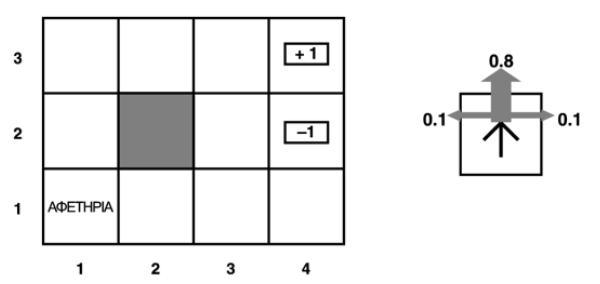
\includegraphics[width=80mm]{grid_world}
	\caption{3x4 grid world and transition model \label{overflow}}
\end{figure}
	
	

	In case there is a wall in the direction that the agents wishes to move, then it stays put.
	The agent is in constant feedback loop with the environment meaning it takes an action $\alpha$ in state s and lands in a stochastic manner in state s’ and gets a reward r'.
	
	The above desicion making problem can be formulated mathematically using Markov Decision Process which will discuss in next section.
	
	\section{Markov Decision Process (MDP)}
	
	Markov Decision process can formally describe the interaction between an agent and the environment. MDPs rely on so-called Markov property, which states that the future is independent of the past given the current/present state. Intuitevely, markov property tells us that all information gathered from previous states can be consider as irrelevant as the information of the current state is sufficient. We can formulate this definition as:
	
	A state $s$ has a Markov property if for all states $\forall{s'} \in S$ and all rewards $r \in R$
	
	\begin{equation}
		\begin{split}
			p(R_{t+1} = r , S_{t+1}=s' | S_{t=s}) = \\ 
		 	p(R_{t+1} = r , S_{t+1}=s' | S_{1} ... S_{t-1}, S_{t})
		\end{split}
	\end{equation}
	for all possible histories $ S_{1} ... S_{t-1}, S_{t} $
	
	In Markov decision process problems the goal is to find an optimal policy $\pi$* that gives  the best action for each state. Optimal policy $\pi$* maximizes the expected sum of discounted(or not) rewards. The reward and discount factor together define what it means to be optimal in an MDP framework.
	
	An MDP is defined by the following components:
	\begin{enumerate}
		\item Set of possible states: $S = \{ s_{0}, s_{1}, ..., s_{n} \}$
		\item Initial state: $S_{0}$
		\item Set of possible actions: $A = \{ a_{1}, a{2}, ..., a_{m} \}$
		\item Transition model: $T(s, a, s')$
		\item Reward function: $R(s)$
		\item $\gamma \in [0,1] $ is the discount factor
	\end{enumerate}

	In its general form, the agent operates in a stochastic environment thus we model the non-determistic process with a transition model such as $T(s,a,s')$. However, in real world applications such a model is unknown, the agent does not know state transition probabilities or rewards and it could only discover them by taking an action on certain state and receive the reward of the landed state. This approach is called Q-Learning and it a model-free learning. The discount factor $\gamma$ trades off the later rewards to earlier ones. Expected discounted reward is defined as:
	
	\begin{equation}
		\mathbb{E}[R | s,a] = \sum_{r}r \sum_{s'}p(r, s' | s, a)
	\end{equation}
	
	while the expected utility of each state is:
	
	\begin{equation}
		U(s) = \mathbb{E}[ \sum_{i}\gamma^{i}R(s_{i})]
	\end{equation}
	
	
	and the total utility is:
	
	\begin{equation}
		U([s_{0}, s_{1}, .... s_{i}, ....] = \sum_{i}\gamma^{i}R(s_{i})
	\end{equation}
	
	\section{Value Iteration}
	Value iteration or Bellman update is a recursive dynamic programming algorithm. It is a method of computing the best values for each possible state an agent can be and eventually extracting the optimal policy $\pi$* for an MDP problem. The agent takes an action $\alpha$ from state s and it lands in state s’ with a probability as this given by transition model. Consider the grid world we have shown above. The reward of state $R(\big \langle 3,4 \big \rangle) = 1$ while $R(\big \langle 2,4 \big \rangle) = -1$. The Bellman update equation is given below.
	
	\begin{equation}
		V(s) \leftarrow \max_{a} { ( R(s,a) + \gamma \sum_{s'}T(s,a,s')V(s') )}
	\end{equation}
	
	Intuitively, the value of V(s) is the best action that maximizes the expected reward. In order to compute the value state of cell(3,3) we need to calculate all the  future rewards for every possible action $A = \{ a_{1}, a{2}, ..., a_{m} \}$ and then choose the best action. In this example we set discount factor $\gamma = 0.9$ and living reward $R=0$. Breaking down equation (5) we write:
	
	
	\begin{enumerate}
		\item Agent tries to go right: 
		\begin{equation}
			\begin{split}
			V(\big \langle 3,3 \big \rangle)_{right} = \\ 
			\sum_{s'} T(\big \langle 3,3 \big \rangle, right, s') [R(\big \langle 3,3 \big \rangle), \gamma V(s')]
			\end{split}
		\end{equation}


		\begin{equation}
			\begin{split}
				V(\big \langle 3,3 \big \rangle)_{right} = 0.9[0.8 * 1 + 0.1 * 0 + 0.1 * 0]
				\end{split}
		\end{equation}

		\begin{equation}
			V(\big \langle 3,3 \big \rangle)_{right} = 0.9[0.8 * 1 + 0.1 * 0 + 0.1 * 0]
		\end{equation}
	
		\begin{equation}
			V(\big \langle 3,3 \big \rangle)_{right} = 0.72
		\end{equation}
		
		\item Agent tries to go left: 
		
			\begin{equation}
			\begin{split}
				V(\big \langle 3,3 \big \rangle)_{left} = \\
				 \sum_{s'} T(\big \langle 3,3 \big \rangle, left, s') [R(\big \langle 3,3 \big \rangle), \gamma V(s')]
			\end{split}
		\end{equation}
		
		
		\begin{equation}
			\begin{split}
				V(\big \langle 3,3 \big \rangle)_{left} = 0.9[0.8 * 0 + 0.1 * 0 + 0.1 * 0]
			\end{split}
		\end{equation}
		
		\begin{equation}
			V(\big \langle 3,3 \big \rangle)_{left} = 0
		\end{equation}
		

	
		\item Agent tries to go down: 
		
				\begin{equation}
			\begin{split}
				V(\big \langle 3,3 \big \rangle)_{down} = \\ 
				\sum_{s'} T(\big \langle 3,3 \big \rangle, down, s') [R(\big \langle 3,3 \big \rangle), \gamma V(s')]
			\end{split}
		\end{equation}
		
		
		\begin{equation}
			\begin{split}
			V(\big \langle 3,3 \big \rangle)_{down} = 0.9[0.8 * 0 + 0.1 * 0 + 0.1 * 1]
			\end{split}
		\end{equation}
		
		\begin{equation}
			V(\big \langle 3,3 \big \rangle)_{down} = 0.09
		\end{equation}
		

		\item Agent tries to go up: 
		
		
		\begin{equation}
			\begin{split}
				V(\big \langle 3,3 \big \rangle)_{up} = \\ 
				\sum_{s'} T(\big \langle 3,3 \big \rangle, up, s') [R(\big \langle 3,3 \big \rangle), \gamma V(s')]
			\end{split}
		\end{equation}
		
		
		\begin{equation}
			\begin{split}
				V(\big \langle 3,3 \big \rangle)_{up} = 0.9[0.8 * 0 + 0 * 0 + 0.1 * 1]
			\end{split}
		\end{equation}
		
		\begin{equation}
			V(\big \langle 3,3 \big \rangle)_{up} = 0.09
		\end{equation}
		
	\end{enumerate}	
		
	Then we take the action that maximizes the value state. 
		
	\begin{equation}
		\begin{split}
		V(\big \langle 3,3 \big \rangle) = \max_{a} [V(\big \langle 3,3 \big 
		\rangle)_{right},V(\big \langle 3,3 \big \rangle)_{left},\\
		 V(\big \langle 3,3  \big \rangle)_{down}, V(\big \langle 3,3 \big \rangle)_{up}]
		\end{split}
	\end{equation}

	\begin{equation}
	 V(\big \langle 3,3 \big \rangle) = 0.72
	\end{equation}


	The above process is repeated for all states. After having calculated all values we repeat again until convergence which is guaranteed by Value iteration algorithm.
	\subsection{Pseudo code}
	Below we present the pseudo code of Value Iteration algorithm.
	\newline
	\newline
	Initialize array V with zeros ( V(s) = 0 )
	\newline
	Repeat:
	\newline
	\tab $\delta \leftarrow 0$
	\newline
	\tab  $\text{For each s} \in S:$
	\newline
	\tab  \tab  $u \leftarrow V(s)$
	\newline
	\tab  \tab  $V(s) \leftarrow \max{ ( R(s,a) + \gamma \sum_{s'}T(s,a,s')V(s') )}$
	\newline
	\tab  \tab  $\delta \leftarrow \max{\delta, | u - V(s)|}$
	\newline
	Until $\delta < \theta$ (small positive number)
	
	
	\subsection{Discount factor}
	 One  important parameter for solving  MDPs is the discount factor $\gamma$. Discount factors are important in MDPs, in a sense they determine how the reward is counted in future states.
	 In this section, we will evaluate the impact discount factor $\gamma$ has, to optimum value $V_{s}^{*}$ of each state s and ultimately to optimal policy $\pi^{*} $ after the convergece of value iteration algorithm. Particularly, given 3x4 world we defined in section I, we will explore the results for 3 different $\gamma$ values, 0.9, 0.6, 0.2 after 100 iterations. Results presented in the table below.
	 
	 	\begin{center}
	 	\begin{tabular}{ c c c c}
	 		\hline
	 		\multicolumn{4}{|c|}{  \text{$\gamma = 0.2$} } \\
	 		\hline
	 		-0.01  & 0.02  & 0.16 & 1.00 \\ 
	 		-0.01  & 0.00  & 0.0  & -1.00 \\  
	 		-0.01 & -0.01 &  -0.01 & -0.01
	 	\end{tabular}
	 \end{center}
	
		\begin{center}
		\begin{tabular}{ c c c c}
						 \hline
			\multicolumn{4}{|c|}{  \text{$\gamma = 0.6$} } \\
			\hline
			0.11 & 0.25 & 0.52 &1.00 \\ 
			0.03 & 0.00 & 0.18 & -1.00  \\  
			-0.01 &  0.0 & 0.06 & -0.04    
		\end{tabular}
	\end{center}

	\begin{center}
	\begin{tabular}{ c c c c}
		\hline
		\multicolumn{4}{|c|}{  \text{$\gamma = 0.9$} } \\
		\hline
		0.55  & 0.69  & 0.84 & 1.00 \\ 
		0.44  & 0.00  & 0.53  & -1.00 \\  
		0.34 &  0.29 & 0.38 & 0.17    
	\end{tabular}
\end{center}

Figure 2 shows the number of iterations required

	\begin{figure}[ht!]
		\centering
		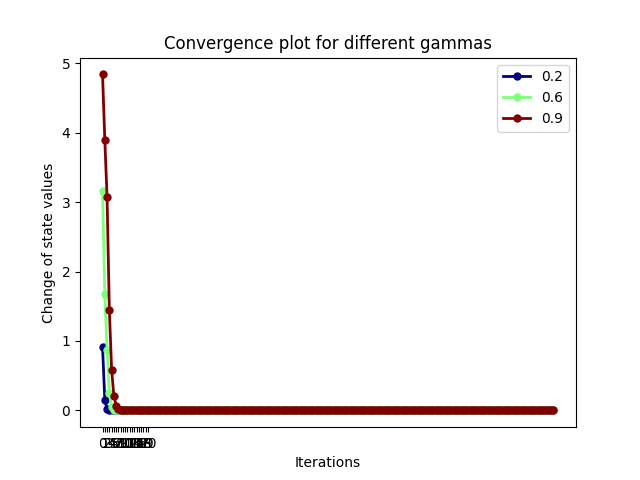
\includegraphics[width=80mm]{gammas}
		\caption{Convergence for $\gamma$ = 0.2, 0.6, 0.9 }
	\end{figure}

	
	Due to trivial problem being discussed in this article, there is no substantial differentiation in number of iterations among different $\gamma$, though there exists some distinction in behaviour which would be magnified in larger problems.

	\section{A* Algorithm}
	A* is a graph traversal and path search algorithm. It differs from Dijkstra as it uses the best first search while taking into account the current cost g and an heuristic function h. It gives priority to nodes that are supposed to be better than others according to the value of function f(s) = g(s) + h(s) where h(s) is a heuristic function. For h(s) = 0, A* is similar to Dijkstra.
	
	The heuristic function is a way to guide the algorithm about the direction it needs to take, in order to find the goal in fewer steps. Usually, the heuristic function emerges from solving the given problem with relaxations about the constraints. We can use any heuristic function for a certain problem as long as it \textbf{consistent} and \textbf{admissible}. Admissible means that the heuristic should never overestimate the actual cost(21), while consistent indicates that the heuristic of predecessor node should be less and/or equal to the sum of the cost and heuristic of successor node (22).
	
	\begin{equation}
		\begin{split}
			\forall n, h(n) \leq g^{*}(n)
		\end{split}
	\end{equation}
	
	
	\begin{equation}
		\begin{split}
			h(s)  \leq g(s,p) + h(p)
		\end{split}
	\end{equation}
	
	where:
	\newline
	\begin{itemize}	
		\item h is the consistent heuristic function
		\item p is any node in the graph
		\item s is any descendant of p
		\item g(s,p) is the cost from p to s
	\end{itemize}
	
	
	Having calculated the optimal values $V^{*}$ for the 3x4 grid world, we will use them as heuristic to find the sortest path from position (1,1) to terminal state with higher reward (3,4). The output of the algorithm is shown in table below. We notice for $\gamma=0.2$ path could not be found.
	
		\begin{center}
		\begin{tabular}{ l l l l l l l }
 		\hline
		\multicolumn{7}{|c|}{  Path taken } \\
		\hline	

			\multicolumn{1}{|l|} {$\gamma=0.9$} & (1,1)  & (2,1) & (3,1)  & (3,2) & (3,3) & (3,4) \\ 
			\multicolumn{1}{|l|} {$\gamma=0.6$}  & (1,1)  & (2,1) & (3,1)  & (3,2) & (3,3) & (3,4) \\ 
			\multicolumn{1}{|l|} {$\gamma=0.2$}  & (1,1)  & - & -  & - & - & - 
		\end{tabular}

	\end{center}

	In the last section, we present $A^{*}$ pseudocode.
	
	\subsection{Pseudo code}
	Below we present the pseudo code of $A^{*}$ .
	\newline
	\newline
	$openlist \leftarrow {0}$
	\newline
	$closelist \leftarrow {0}$
	\newline
	$openlist \leftarrow StartNode$
	\newline
	While 
	
	\section{Conclusion}
	In this article we briefly presented Markov Decision Process problems and the challenge to find the optimal policy for each state an agent could be. We used Value Iteration algorithm to calculate the value of each state and explored the impact of discount factor $\gamma$. Lastly, we implemented A* path finding algorithm and used the converged state-values as heuristic.
	We also provided Python implemantions of the two considered algorithms. $\text{valueiteration.py and astar.py}$.
		
	
	\begin{thebibliography}{9}
		\bibitem{russell} 
		Stuart Russell and Peter Norvig. 
		\textit{Artificial Intelligence: A Modern Approach}. 
		Prentice Hall, Fourth Edition 2020.
		
		\bibitem{russell} 
		Casey C.Bennett and Kris Hauser. 
		\textit{Artificial intelligence framework for simulating clinical decision-making: A Markov decision process approach}. 
		Elsevier, January 2013.
		
		\bibitem{Hasselt} 
		van Hasselt, H., Guez, A., and Silver, D. (2016). 
		\textit{Deep Reinforcement Learning with Double Q-Learning}. 
		Proceedings of the AAAI Conference on Artificial Intelligence, 30(1). 
		

	\end{thebibliography}
	

\end{document}